\documentclass{article}
\usepackage{tabularx,fullpage,url}
\usepackage[top=1in, bottom=1in, left=.5in, right=.75in]{geometry}
\usepackage{amsmath,amssymb,graphicx,amsthm,xparse, color, mathrsfs} 
\usepackage{ epstopdf, fullpage}

\usepackage[ruled,vlined]{algorithm2e}
\usepackage{xifthen}
\usepackage{wrapfig}

\newcommand{\mypagebreak}{\begin{center}
		\noindent\makebox[\linewidth]{\rule{7.5in}{1pt}}
	\end{center}}
\bibliographystyle{siam}
\newcommand{\minimize}[1]{\underset{#1}{\text{minimize}}}
\newcommand{\maximize}[1]{\underset{#1}{\text{maximize}}}
\newcommand{\mini}[1]{\underset{#1}{\text{min}}}
\newcommand{\argmin}[1]{\underset{#1}{\text{argmin}}}
\newcommand{\st}{\text{subject to}}
\newcommand{\rank}{\textbf{rank}}
\newcommand{\epi}{\mathbf{epi}}

\newcommand{\diag}{\textbf{diag}}
\newcommand{\mb}{\mathbf}
\newcommand{\R}{\mathbb R}
\newcommand{\mle}{\mathbf{MLE}}
\newcommand{\map}{\mathbf{MAP}}
\newcommand{\bE}{\mathbb E}
\newcommand{\mL}{\mathcal L}
\newcommand{\mH}{\mathcal H}
\newcommand{\mB}{\mathcal B}
\newcommand{\mN}{\mathcal N}
\newcommand{\mD}{\mathcal D}
\newcommand{\mC}{\mathcal C}

\newcommand{\mS}{\mathcal S}
\newcommand{\tr}{\mathbf{tr}}
\newcommand{\mrm}{\mathrm}
\newcommand{\proj}{\mathbf{proj}}
\newcommand{\prox}{\mathbf{prox}}
\newcommand{\sign}{\mathbf{sign}}
\newcommand{\range}{\mathbf{range}}
\newcommand{\var}{\mathbf{var}}
\newcommand{\vnull}{\mathbf{null}}
\newcommand{\pr}{\mathbf{Pr}}
\newcommand{\find}{\mathbf{find}}
\newcommand{\argmax}[1]{\underset{#1}{\mathrm{argmax}}}
\newcommand{\subjto}{\mathrm{subject~to}}


\newcommand{\red}[1]{{\color{red}#1}}
\newcommand{\blue}[1]{{\color{blue}#1}}

\newcommand{\gray}[1]{\textcolor{lightgray}{#1}}



\newcommand{\idx}[1]{{\scriptsize [#1]}}

\newcommand{\showpoints}[1]{\textbf{(#1)}}

 
\begin{document}
{\Large\textbf{CSE 353: Homework  2 Solutions \hfill
Due Friday September 23}}


\mypagebreak



\begin{center}
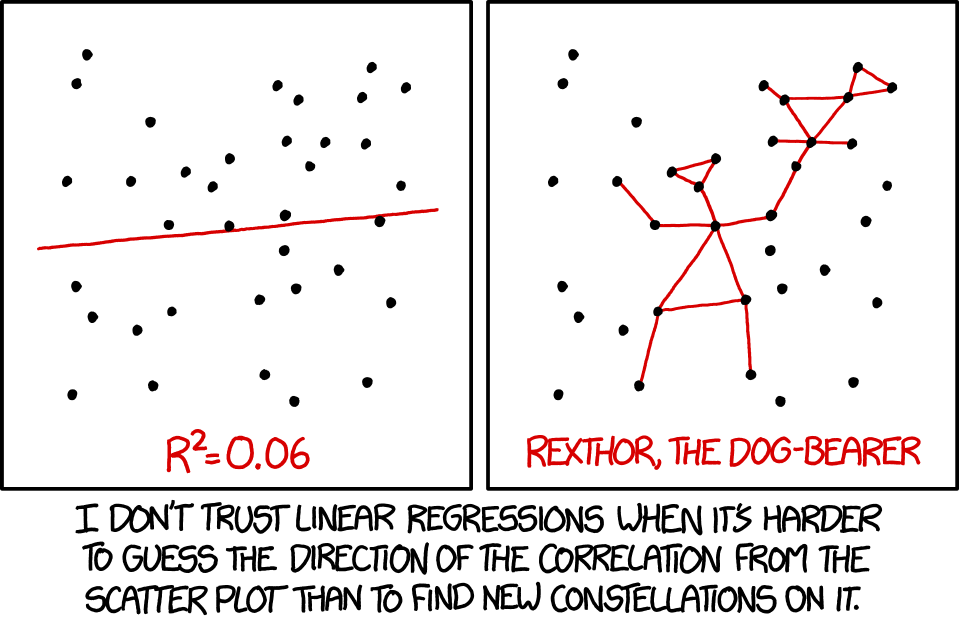
\includegraphics[width=.5\linewidth]{figs/overfit.png}\\
(credit: xkcd)
\end{center}
\begin{enumerate}
\item \showpoints{3 pts, 1 pt each} \emph{Machine learning fundamentals.} In the following scenarios, discuss whether or not you believe that I did a good job in \emph{model generalization.} Justify your answer.



\begin{enumerate}
\item I work in real estate. I have observed, over 10 years of experience, that large houses on Long Island tend to sell at around \$500,000 or more, while small houses sell at around \$400,000 or fewer. I move to the Texas Panhandle, and find a house that is very large, and conclude that it should be worth around \$500,000 or more.



\item I am a young upshot professional and I would love to live in New York City. I talk to my friend, who lived in NYC in the late 2000's, and she tells me    how factors affect rent prices (quality of apt, number of bedrooms, neighborhoods, allow pets, etc.)   The year is now 2020. Does her advice generalize to my current situation? (Hint: Think COVID.)



\item I am a computer science expert who has spent the past 5 years classifying images of dogs and cats. I'm pretty good at this now, and my 1 million layer neural network achieves 100\% accuracy (in testing and training) on this task. Now, the government wants me to apply my neural network to remote sensing satellite images, to detect underground marijuana farms. I use the same neural network, with no tweaking, on this new task, and expect the same level of accuracy.

\end{enumerate}




\item \showpoints{2 pts, 0.5 points each} \emph{Conditional independence vs independence.} 

\begin{tabular}[t]{lll}
\begin{minipage}{.75\linewidth}
Tom is a blue-gray cat with a bushy tail, and Jerry is a brown mouse with a rope-like tail. After many years of fighting, they both decided to settle down, and now have thriving families. Tom has 10 kids and Jerry has 40 kids. Tom's kids are all  cats like him, with bushy tails. Half of Tom's kids are blue, while the other half is gray. Jerry's kids are all brown mice, with rope-like tails.
\end{minipage}
&$\quad$&
\begin{minipage}{.2\linewidth}

\includegraphics[width=\linewidth]{figs/tomjerry.jpg}

\end{minipage}
\end{tabular}


\begin{enumerate}
\item 
I pick up a baby animal at random.  What is the probability that ... (fill in the table)
\begin{center}
\begin{tabular}{|l|ll|}
\hline
fur $\backslash$ tail & furry & rope-like\\\hline
&&\\blue&&\\&&\\
&&\\gray&&\\&&\\
&&\\brown&&\\&&\\
\hline
\end{tabular}
\end{center}



\item Are the features ``fur color" and ``tail texture" independent or dependent, without knowing the type of animal? (Show mathematically.)



\item Now Tom comes over and says, ``I'm very proud of my baby girl, of whom you are holding."
 What is the probability that  (fill in the table)
\begin{center}
\begin{tabular}{|l|ll|}
\hline
fur $\backslash$ tail & furry & rope-like\\\hline
&&\\blue&&\\&&\\
&&\\gray&&\\&&\\
&&\\brown&&\\&&\\
\hline
\end{tabular}
\end{center}



\item Are the features ``fur color" and ``tail texture" independent or dependent, now that I know the animal is Tom's cherished baby daughter? (Show mathematically.)


\end{enumerate}




\item \showpoints{2pts} \emph{Directed graphical models and probability inference} 
I have 4 tops: a red sweater, a blue T-shirt, a green hoodie, and a white tank top.
I need your help to decide what to wear.

\begin{enumerate}

\item I decide what to wear based on four factors:
\begin{itemize}
\item if it's raining
\item if I want to take a walk outside
\item if I feel sick
\item the day of the week it is
\end{itemize}

%\begin{center}
%\begin{tabular}{l|llll}
%& red sweater & blue T-shirt & green hoodie & white tank top\\\hline
%raining & 40\% & 10\% & 40\% &10\%\\
%walking outside & 35\% & 5\% & 60\% & 0\%\\
%I feel sick & 5\% & 5 \% & 80\% & 10\%\\
%It's Monday & 80\% & 5\% & 10\% & 5\%
%\end{tabular}
%\end{center}

\showpoints{0.5pts} Using the Naive Bayes assumption, draw a graphical model that indicates how I will make a decision of what to wear each day.


\item \showpoints{1pt}  To be more specific, 
\begin{itemize}
\item I only wear the green hoodie when I walk outside, regardless of all other factors. 
\item If I feel sick, I will walk outside 10\% of the time. If I feel well, I will walk outside 60\% of the time.
\item When it rains, I feel sick 70\% of the time; otherwise, I feel sick 15\% of the time.
\end{itemize}
Draw a corresponding graphical model for determining whether I wear a green hoodie. Given that it is raining, infer the probability that I am wearing a green hoodie.





\item \showpoints{0.5pts}  The probability that I wear a tank top, independently of all the other clothes, is 75\% if it's raining and 25\% if it's not raining.
\begin{itemize}
\item
Today is Monday and it is raining.

\item 
The probability that it will rain, given that the previous day rained, is 70\%. The probability that it will rain, given that the previous day did not rain, is 10\%. 

\end{itemize}
Draw a graphical model predicting whether I will wear a tank top on Wednesday, and calculate this probability.



\end{enumerate}



\item  \showpoints{3 pts}  \textbf{Naive Bayes  and Alice in Wonderland.}

\begin{itemize}

\item Our goal is now to do word prediction, using the $n$ preceding words as $n$ features for each word. As an example, consider the following text
\begin{center}
\texttt{The quick brown fox jumped over the fence}
\end{center}

Then, if $n = 1$, our training data will be formed as

\begin{center}
\begin{tabular}{r||c|c|c|c|c|c|c}
features & the & quick & brown & fox & jumped & over & the\\\hline
label & quick & brown & fox & jumped & over & the & fence.
\end{tabular}
\end{center}
If $n = 2$, our training data will look like

\begin{center}
\begin{tabular}{r||c|c|c|c|c|c}
features &  the, quick & quick,brown & brown,fox & fox,jumped & jumped,over & over,the\\\hline
label &  brown & fox & jumped & over & the & fence.
\end{tabular}
\end{center}

and so forth.


That is, if we think of each task as taking a list of features and spitting out a label, then 

\item Open the python notebook \texttt{hw2\_alice\_naivebayes\_release.ipynb} . After running the first couple boxes, you should have loaded the entire text of ``Alice in Wonderland" by Lewis Caroll, as an ordered list of words. Our task today will be to do word prediction based on this corpus. Throughout this exercise, this corpus will serve as both our training and testing data. 

\item \textbf{Tokenize} While the exact word means a lot to us, for a (primitive) computer, a word is just some object; in particular, we represent each unique word as a unique number. This is the word's token. Run the 3rd block to tokenize the data, and understand what it is doing. 

\item \textbf{Counting of past words.} In the next box, I give you code that generates a lookup table, which counts how many times a word precedes a previous word. This matrix is then $V\times V$ where $V = 2637$ is the number of distinct words. Each row of that matrix is indexed by $y$ the label, and each column by $x$ the feature.

\item[(a)]\showpoints{1 pt}  \textbf{Bigram classifier}. Use the table given to create a bigram classifier, e.g. predicting the next word using only the previous word ($n=1$). That is, construct a calculation for the posterior $\pr(x|y)$ and the prior $\pr(y)$ based on the statistics of the corpus. Do not worry about normalization, e.g. the likelihood function can return the first term of
\[
\pr(x|y)\pr(y)\propto \pr(y|x).
\]
Now construct a Bayes classifier using only this feature.
To check your work, the following words should be the highest likely bigrams.

\begin{itemize}
\item 
word: \texttt{alice}. Most frequent previous word: \texttt{said}, with probability $0.00534$.

\item 
word: \texttt{the}. Most frequent previous word: \texttt{said}, with probability $0.00233$.

\item 
word: \texttt{cat}. Most frequent previous word: \texttt{the}, with probability $0.0396$.


\item 
word: \texttt{turtle}. Most frequent previous word: \texttt{mock}, with probability $0.00221$.


\end{itemize}

 \textbf{Report the classification accuracy} over the entire corpus of this classifier.


\item[(b)] \showpoints{0.5 pts}   Well, that was pretty terrible. Let's try and incorporate not just the past word, but the past $k$ words, where $k$ can be up to 30. (You can use a tensor and a loop to do this.) Using the code given as a guide, construct more tables that records the counts for how often a word is 2 tokens before another word. Use this to fill in the posterior for $\pr(x|y)$ where now $x$ is the 2nd previous word. 
 Now construct a Naive Bayes classifier that uses both the past and past 2nd word as features. Remember that using the Naive Bayes assumption,
 
\[
\pr(y|x_1,x_2) \propto \pr(x_1,x_2|y) = \pr(x_1|y)\pr(x_2|y). 
\] 
Make sure that your model respects this independence.
Here are some sanity checks:
\begin{itemize}
\item seed: \texttt{'before', 'she', 'found', 'herself', 'falling', 'down', 'a', 'very', 'deep'}.  Next most likely word: \texttt{well}, with probability 0.00276

\item seed: \texttt{'what', 'an', 'ignorant', 'little'}.  Next most likely word: \texttt{shoulders}, with probability 0.000474

\item seed: \texttt{'four','thousand'}. Next most likely word: \texttt{miles}, with probability 0.000118
\end{itemize}
  
  \textbf{Report the classification accuracy} over the entire corpus of this classifier, for $n = 3, 5, 10$. (Note that this is not an $n$-gram classifier, which would be the not-Naive-Bayes version of what we are doing here.)



\item[(c)]  \showpoints{0.5 pts} \textbf{Text generation} Using the likelihoods computed from the  classifier using $n =3$ (3 past words), and starting with a seed phrase ``the mad hatter", generate the next 25 words by always picking the \emph{most likely} next word.



\item[(d)]  \showpoints{1 pt} \textbf{Text generation} Using the likelihoods computed from the $n = 3$  classifier, and starting with a seed phrase ``the mad hatter", generate the next 25 words by always picking the next word \emph{by sampling according to that probability.} (Hint: use \texttt{random.choices()}.)





\end{itemize}






\end{enumerate}

\end{document}